\documentclass[twoside]{jarticle}

\usepackage{grares}
\usepackage[dvipdfmx]{graphicx}
\usepackage{amsmath,amssymb}

\title{Deterministic Interleaver Design for Turbo Codes}
\name{Bohulu Kwame Ackah}
\srnum{1631133}
\bib{主任指導教員~~韓 承鎬~~~~指導教員~~橋本 猛}
\adviser{橋本 猛{Information Transmission Laboratory}}
\date{\today}
\PAGE{3}
\begin{document}
\MKTITLE

%%%%%%%%%%%%%%%%%%%%%%%%%%%%%%%%%%%%%%%%%%%%%%
\section{Introduction}
\vspace{-2mm}
The construction of a turbo code is usually done by the parallel concatenation of two
convolutional codes via an interleaver. The good BER performance of turbo codes is attributed to the interleaver. Interleavers are 
generally grouped into random and deterministic interleavers.  Deterministic interleavers perform interleaving via 
algorithms. For long frame sizes a deterministic interleaver that outperforms the random interleaver is yet to be found.In this research, we attempt to design a deterministic interleaver which performs as well as the random interleaver especially for long interleaver frame sizes.

%%%%%%%%%%%%%%%%%%%%%%%%%%%%%%%%%%%%%%%%%%%%%%
\section{System Model}
\subsection{Encoding and Decoding}
\vspace{-2mm}
\begin{center}
\begin{figure}[h!]
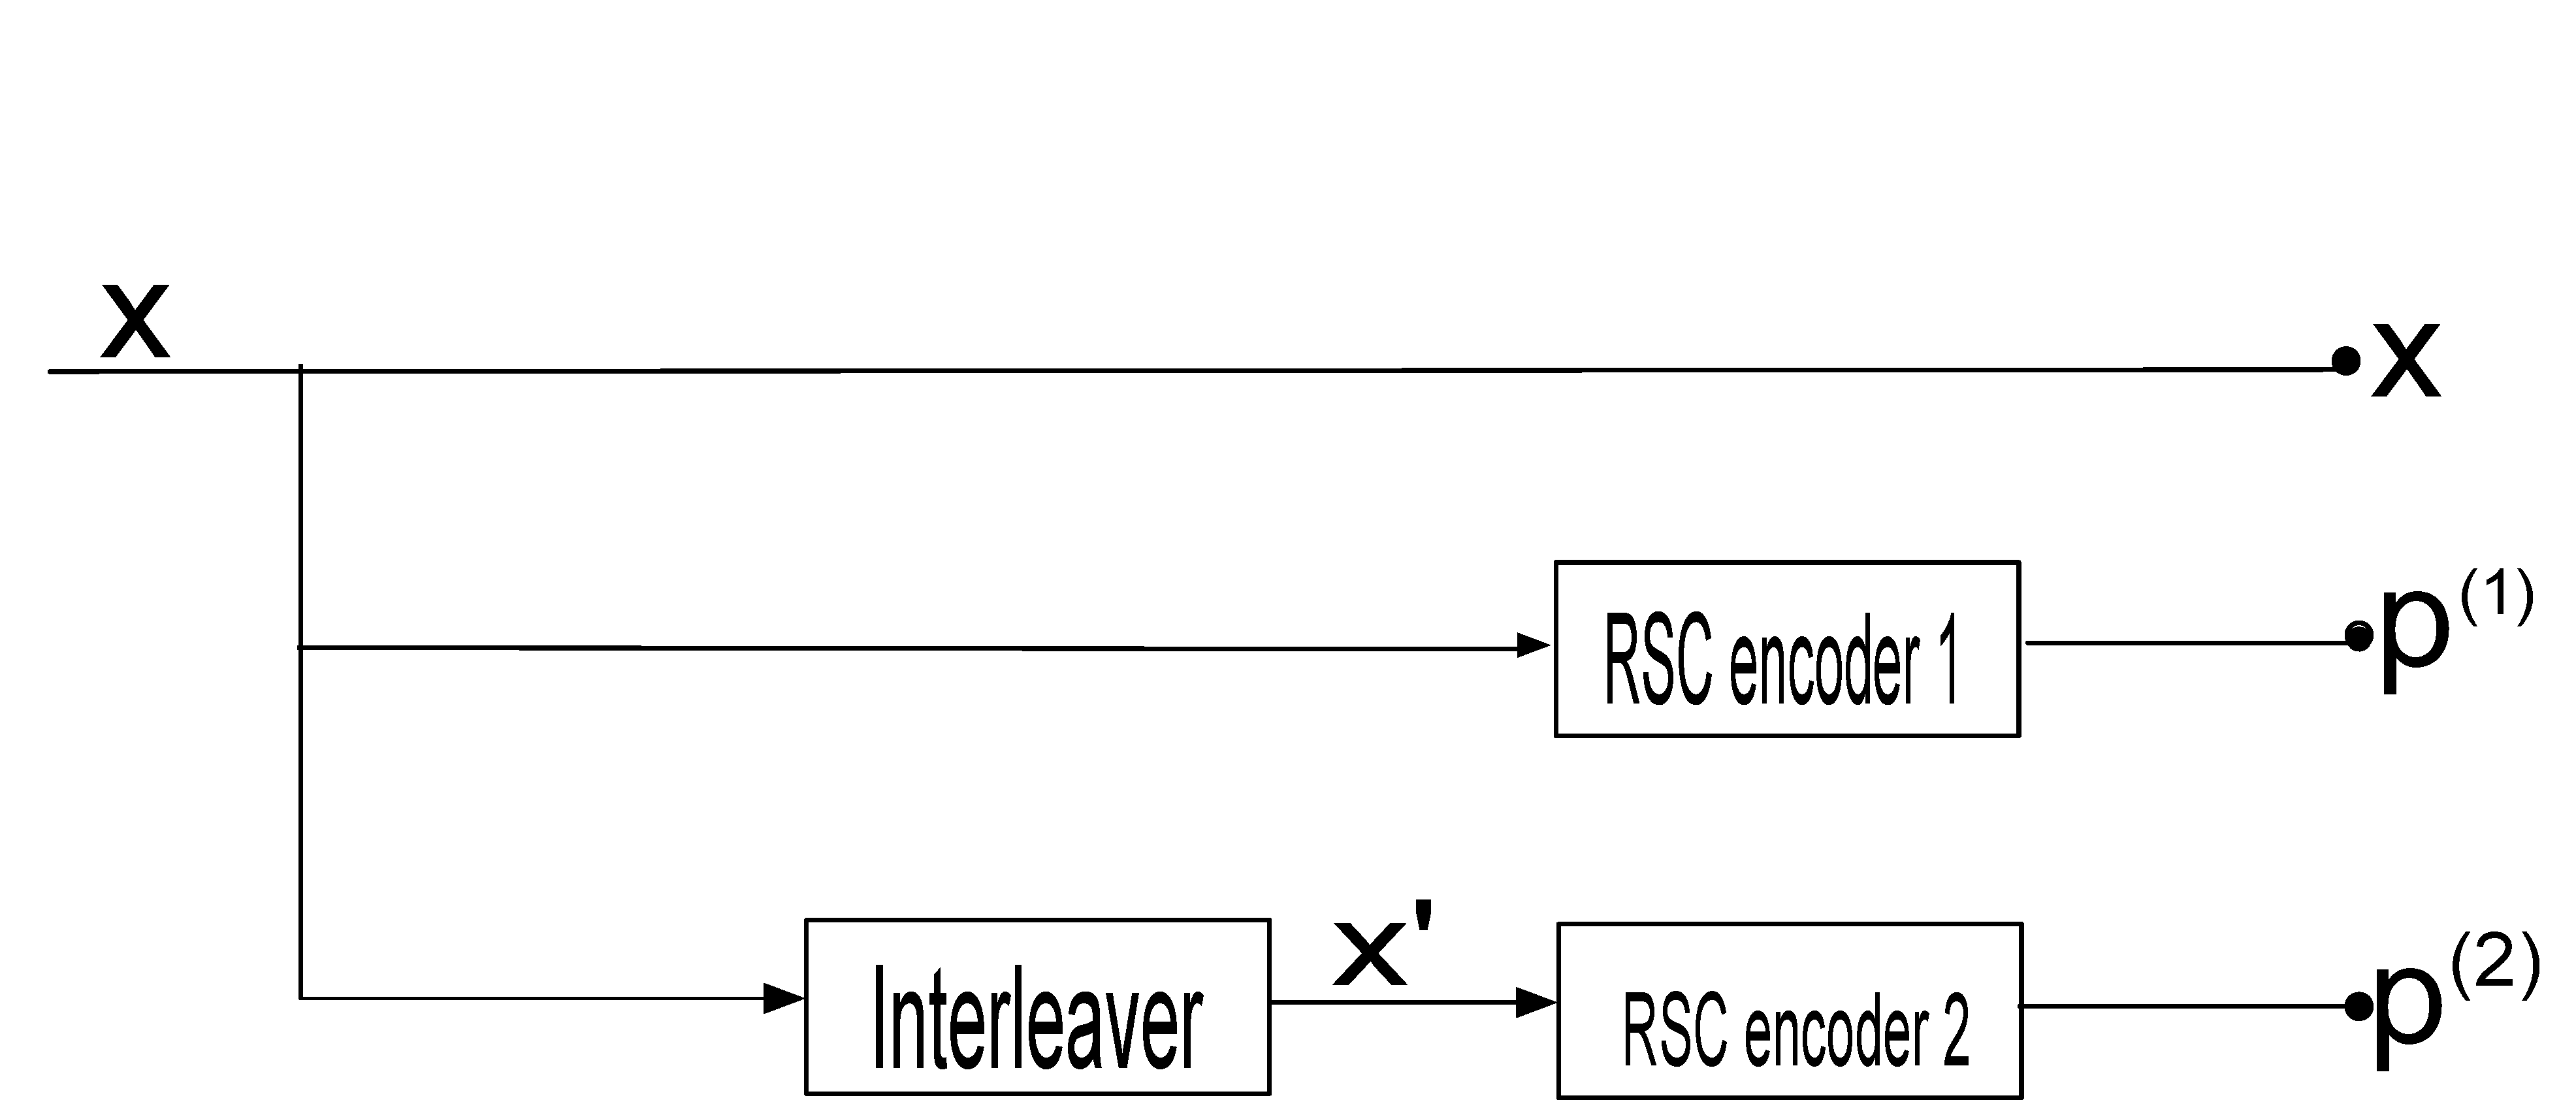
\includegraphics[width=6cm]{TurboEncoder.eps}
\caption{Turbo Encoder}
\label{TC}
\end{figure}
\end{center}
\vspace{-6mm}
The system diagram for the turbo encoder is shown in figure \ref{TC}.
 It is made up of identical Recursive Systematic Convolutional (RSC) encoders which 
 are connected
  in parallel via an interleaver. The RSC encoders have constraint length $K$ and output
  $n$ bits for every $k$ bits input at time $t$.
  From here onward we refer to the RSC encoders as component 
encoders (CE). An information sequence $\mathbf{x} $ of length $N-M$ is fed into the CE1, where $M=K-1$. $M$ tail-bits are added to return CE1 to the all-zero state.  $\mathbf{x}$ and the $M$ tail-bits are used to produce the upper parity check bits  
$\mathbf{p}^{(1)}$ of length N. $\mathbf{x}$ and the $M$ tail-bits are then fed into the interleaver. The interleaved information sequence $\mathbf{x'}$ of length$N$ is then fed into CE2 to produce $\mathbf{p}^{(2)} $ of length $N$. $\mathbf{x}$ (with extra tail-bits), $\mathbf{p}^{(1)}$
 and $\mathbf{p}^{(2)}$ are multiplexed, BPSK modulated and transmitted over the
 AWGN channel. At the receiver, the received signal  $\mathbf{y}$ is split into 
  $\{\mathbf{y}^x,\mathbf{y}^{p^{(1)}},\mathbf{y}^{p^{(2)}}\}$ 
 , where $\mathbf{y}^x,\mathbf{y}^{p^{(1)}},\mathbf{y}^{p^{(2)}}$
    correspond to the systematic, upper and lower parity sequence respectively. These inputs are fed into the Turbo Decoder which performs an iterative decoding process based on the Max-Log-MAP algorithm. Finally, an estimation is made to determine the transmitted information bit sequence.
    
  \subsection{RSC encoders and $\tau$-seperated weight error events}
\begin{figure}[h!]
\centering
		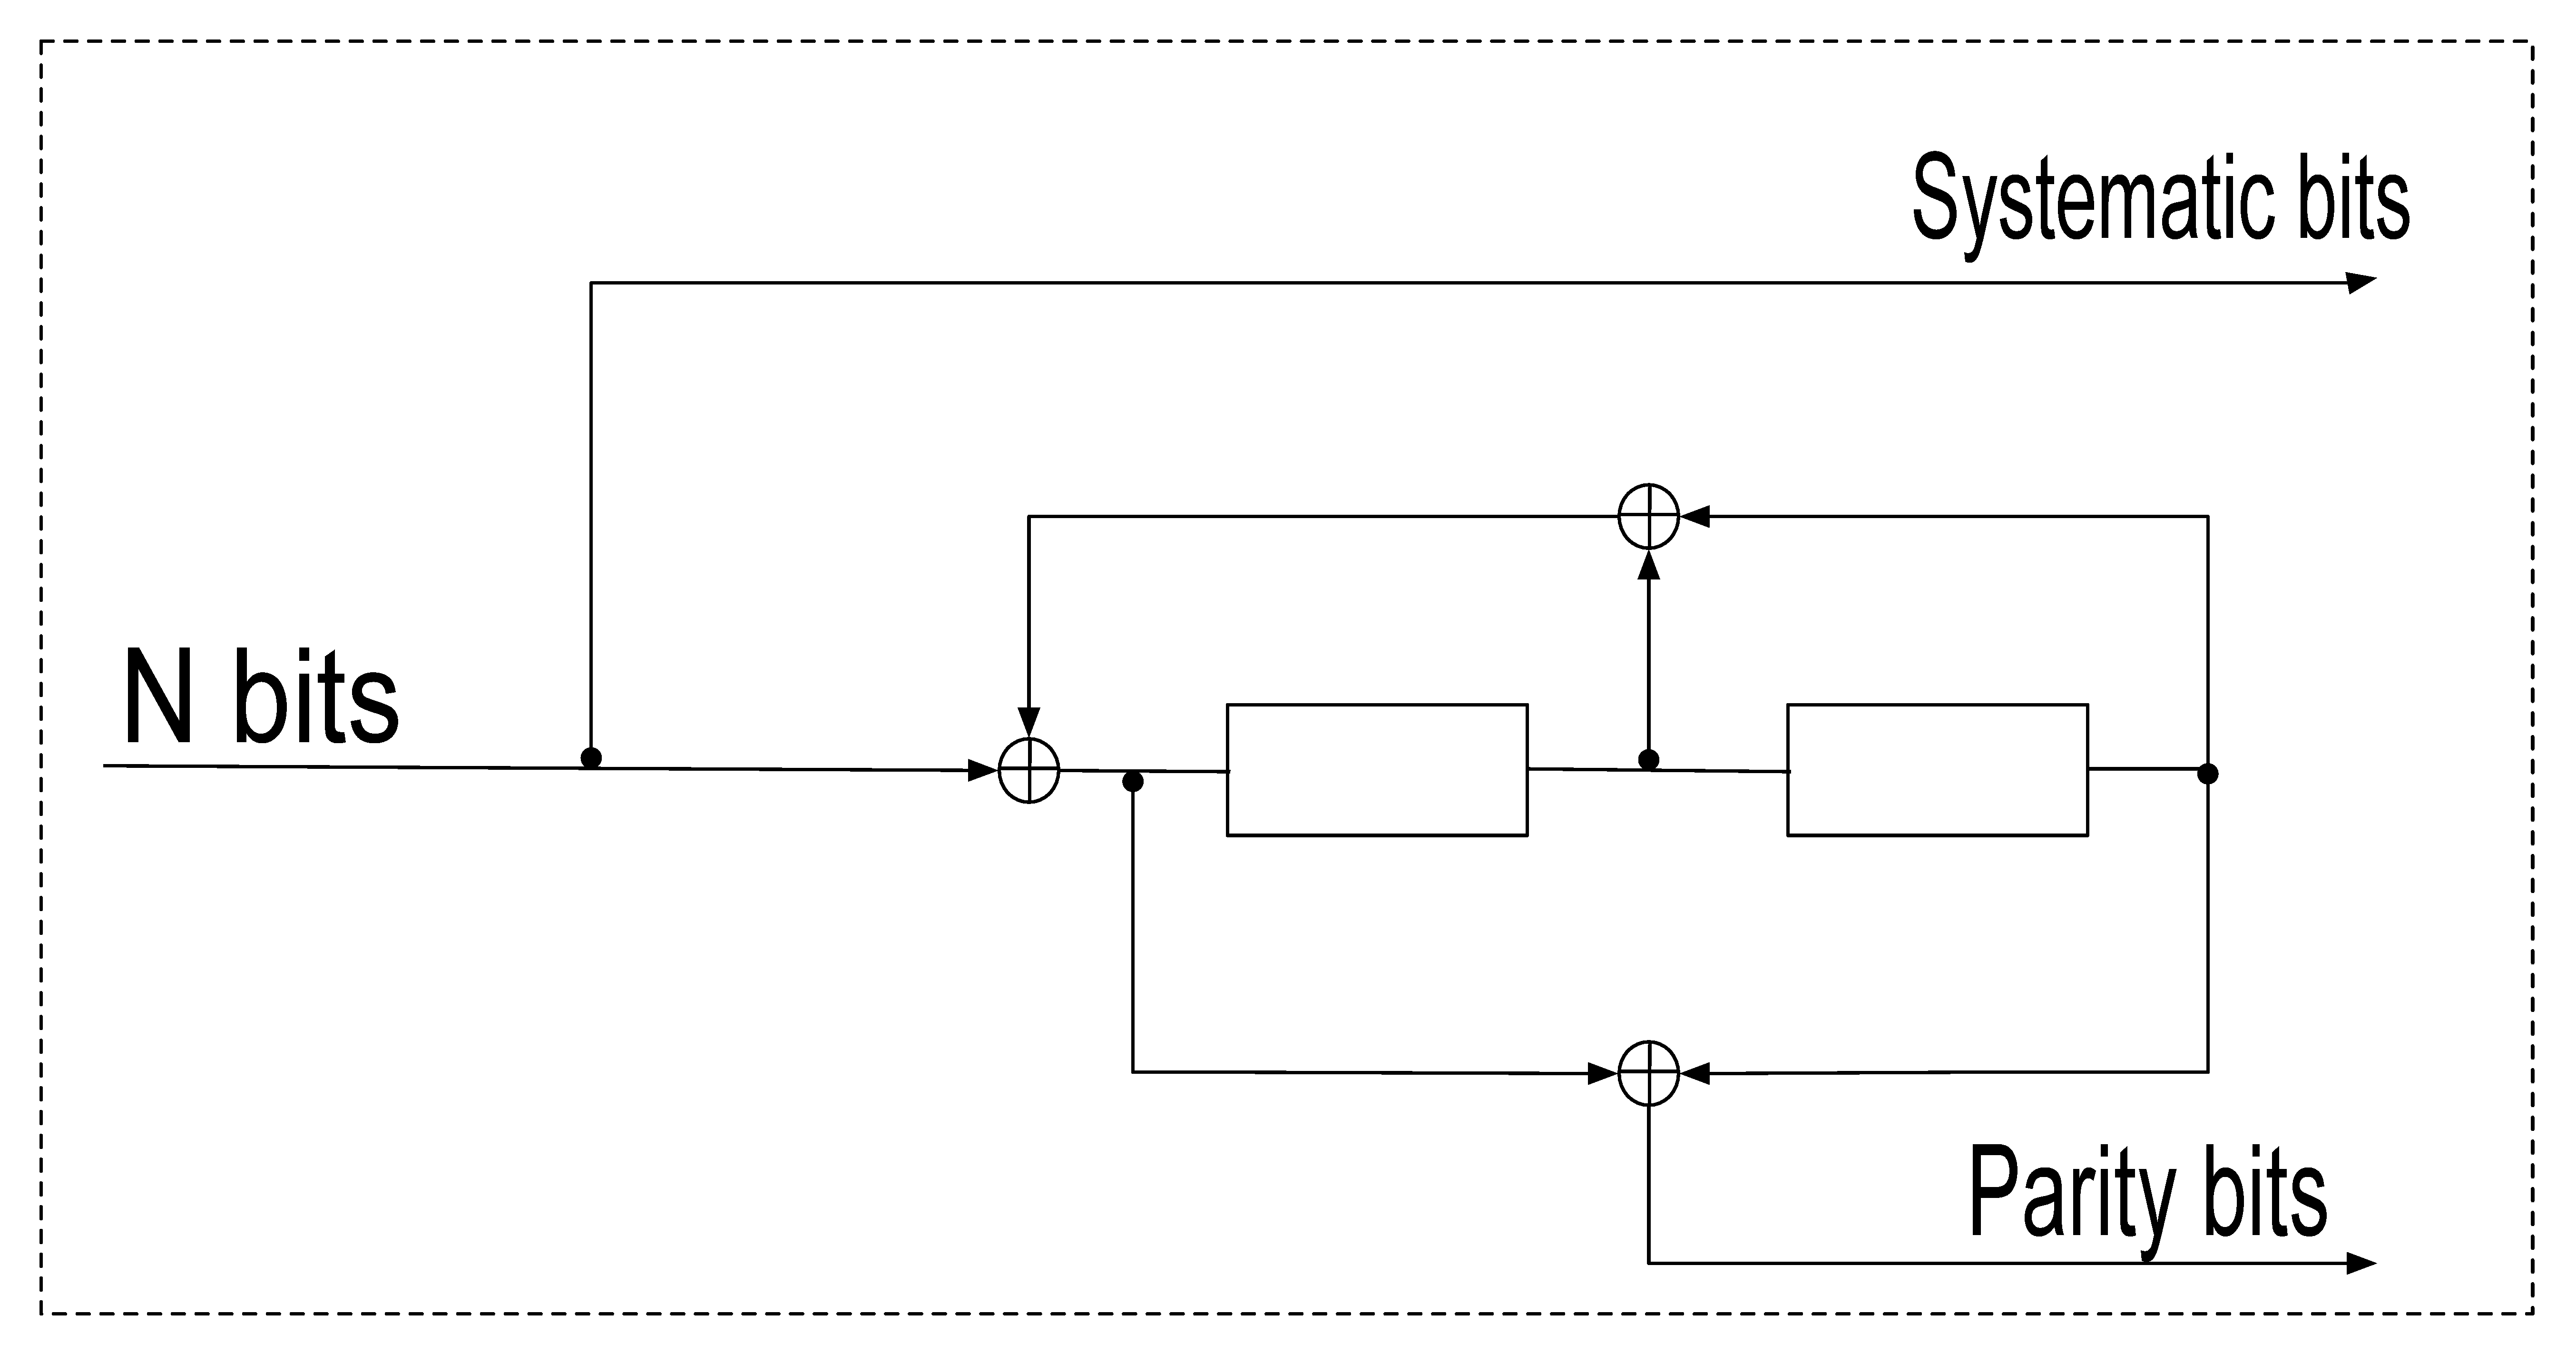
\includegraphics[width=5.0cm]{RSCExample3.eps}
		\caption{$[\frac{1+D^2}{1+D+D^2}]$ (5/7) RSC Encoder}
		\label{RSC}
		\end{figure}
RSC encoders  are
characterized by their cycle length ($\tau$) which is defined as the length of the cycle
 of the parity output of the encoder when the input $\mathbf{x}$ is $[1,0,0,0,....]$[5]. 
For example, the RSC encoder in figure (\ref{RSC})has a parity output $\mathbf{y}$ of 
$[1,1,1,0,1,1,0,1,1,0,...]$. The cycle is $[1,1,0]$ and
the cycle length $\tau=3$. With the knowledge of the cycle and the cycle length $\tau$
of the RSC encoder we wish to explore the effect of weight-$2m$ inputs where the pair of
``1'' bits
 are seperated by $\tau-1$ ``0'' bits. We shall refer to to these inputs as
 $\tau$-seperated weight-$2m$ input error events (or simply as $\tau$ weight-$2m$ errors for
 simplicity sake ), where $m=\{1,2,...\}$. 
In general, the minimum codeword weight associated with weight 2 inputs is known as the effective free distance $(d_{eff})$\cite{ref5}
 Figure(\ref{RSC3})  shows the effect of $\tau$ weight-2 errors on the codeword weight.
 
\begin{figure}[h!]
\centering
		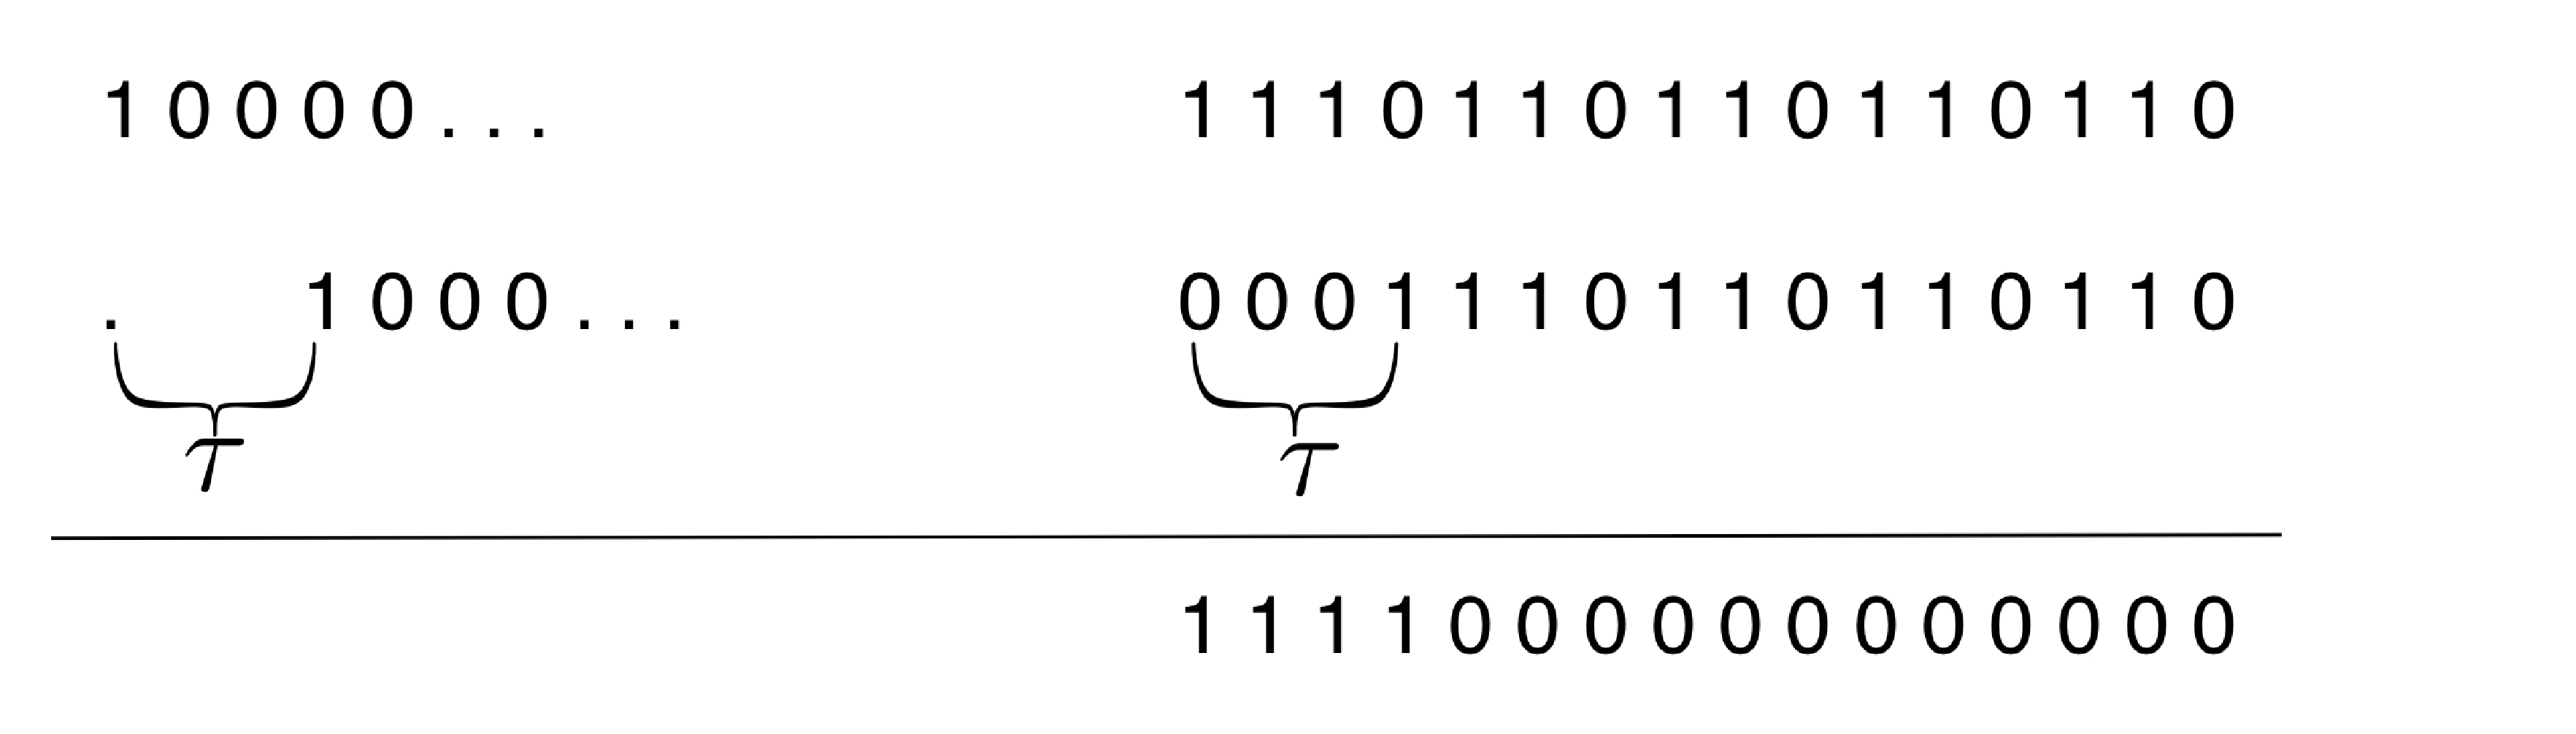
\includegraphics[width=6cm]{RSCExample.eps}
		\caption{ effect of $\tau$ weight-2 errors}
		\label{RSC3}
		\end{figure}
	
 It can be seen that  $\tau$ weight-$2m$ errors result in a low-weight parity output, which inturn results
in a low-weight parity codeword. 
 From the above example, we see that $\tau$ weight-$2m$ errors have the potential to
produce low weight codeword with high multiplicity if they are present in both 
component encoders of the turbo encoder. 
\vspace{-4mm}
%%%%%%%%%%%%%%%%%%%%%%%%%%%%%%%%%%%%%%%%%%%%%%
\section{Interleaver Design for Turbo Codes}
\begin{center}
\begin{figure}[h!]
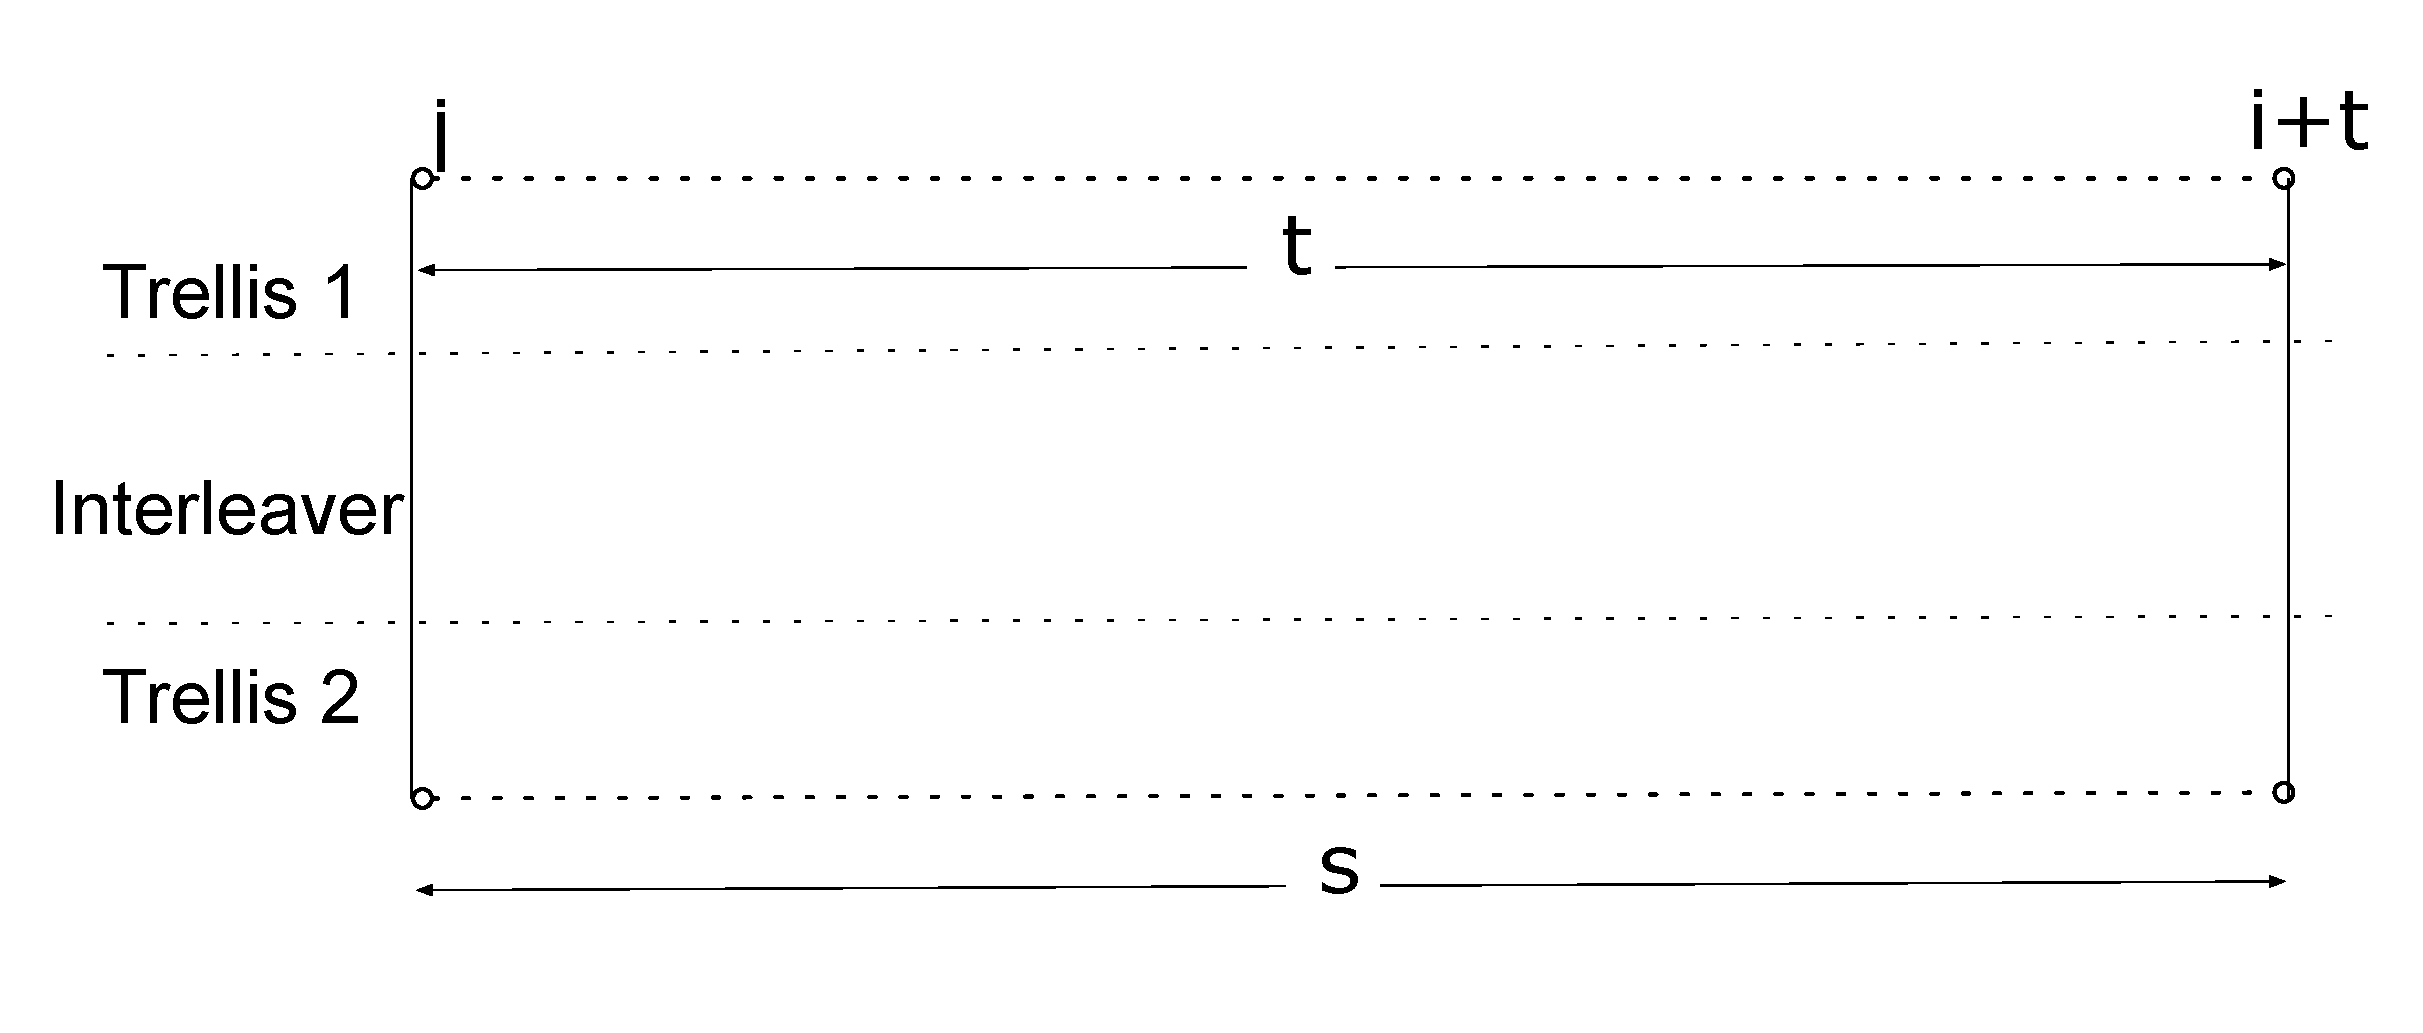
\includegraphics[width=6cm]{weight2.eps}
\caption{$\tau$ weight-$2$ error }
\label{2_error}
\end{figure}
\end{center}
\vspace{-8mm}

\subsection{Linear Interleaver}
The index mapping function of the  linear interleaver is given by 
$ \Pi_{\mathfrak{L}_N}(i) \equiv Di \mod N,  \,\,\, gcd(N,D)=1$ .

$D$ is the interleaver depth. $s = Dt \mod N$ is the input - output distance relationship.
When $t=a\tau$ and $s=b\tau$, a low weight codeword may be produced. To prevent this error event from occuring we choose $D$ that produces the largest value of $\min{( t+s)}$ which  corresponds to a large $d_{eff}$ value. We are able to find good interleavers with large $d_{eff}$ values using this procedure. However we realized that for large frame sizes, the performance of the linear interleaver is dominated by $\tau$ weight-$4$ error events which produce lower weight codewords than $d_{eff}$ and also have high multiplicity as $N$ increases

\vspace{-3mm}
\subsection{Multi-Shift Interleaver}
\vspace{-2mm}
The Multi-Shift Interleaver alters the value of $D$ for every position shift.  
We introduce two new variable, the cycle set $\mathbb{D}$ and step size $\Delta s$. 
  The cycle set $\mathbb{D}=\{d_0,d_1,...,d_{V-1}\},\,\,\, V=N/\Delta s, \,\,\,\, d_i=d_{i-1}+\Delta s, \,\,\, d_0=D$. 
  
 For $N=2^r, \,\,\, r\in \{1,2,...\}$, we set $\Delta s = 2^q, \,\,\, q \in \{2,3,...,r-1\}$. The algorithm for the Multi-Shift Interleaver is shown below.
 
   1. $p_0=0$
   
   2. $p_i=p_{i-1}+d_{((i-1) \mod V) } \mod N$
   \vspace{-8mm}
\subsubsection{Search For Good Interleavers}
\vspace{-2mm}
 We first fix the value $d_0$ and determine the elements of the cycle set. For each element in $\Delta s$, we calculate the hamming weight of the 
 turbo codewords due to $\tau$ weight-$2$ errors using the procedure in Figure \ref{RSC3} and record $d_{eff}$.  The value of 
 $\Delta s$ that is chosen is the one that produces the largest value of $d_{eff}$
 for a given value of $d_0$. This is repeated for all odd integer values of $d_0$
  between $(\sqrt{N},N/2)$. The best interleaver is $(d_0, \Delta s)$with  $\max{d_{eff}}$ followed by $\min{\Delta s}$ and lowest multiplicity.
  \vspace{-4mm}
  \section{Results}
    \begin{center}
\begin{figure}[h!]
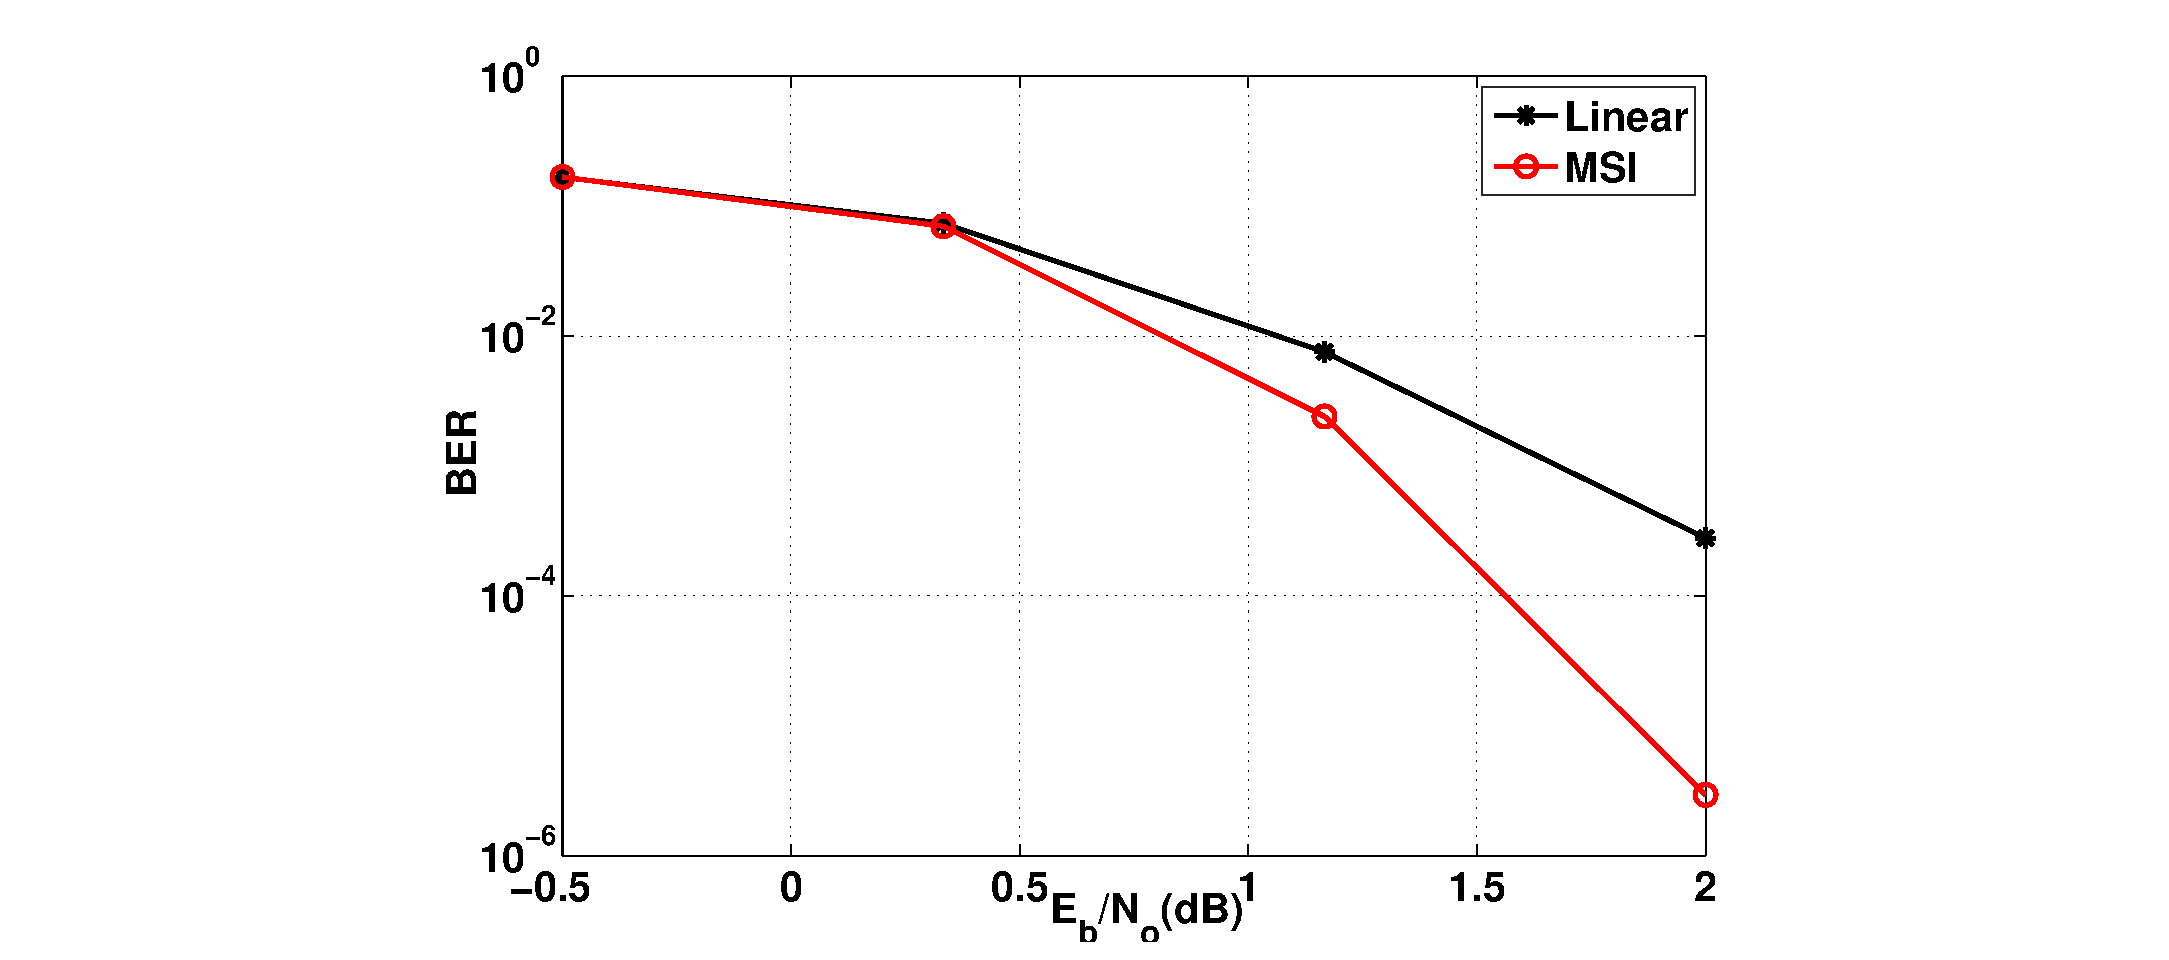
\includegraphics[width=8cm]{msi_linear_256_1000Frames_2.eps}
\caption{$N=1024$, $D = d_0 = 31$ }
\label{x}
\end{figure}
\end{center}
\vspace{-8mm}
\begin{center}
\begin{figure}[h!]
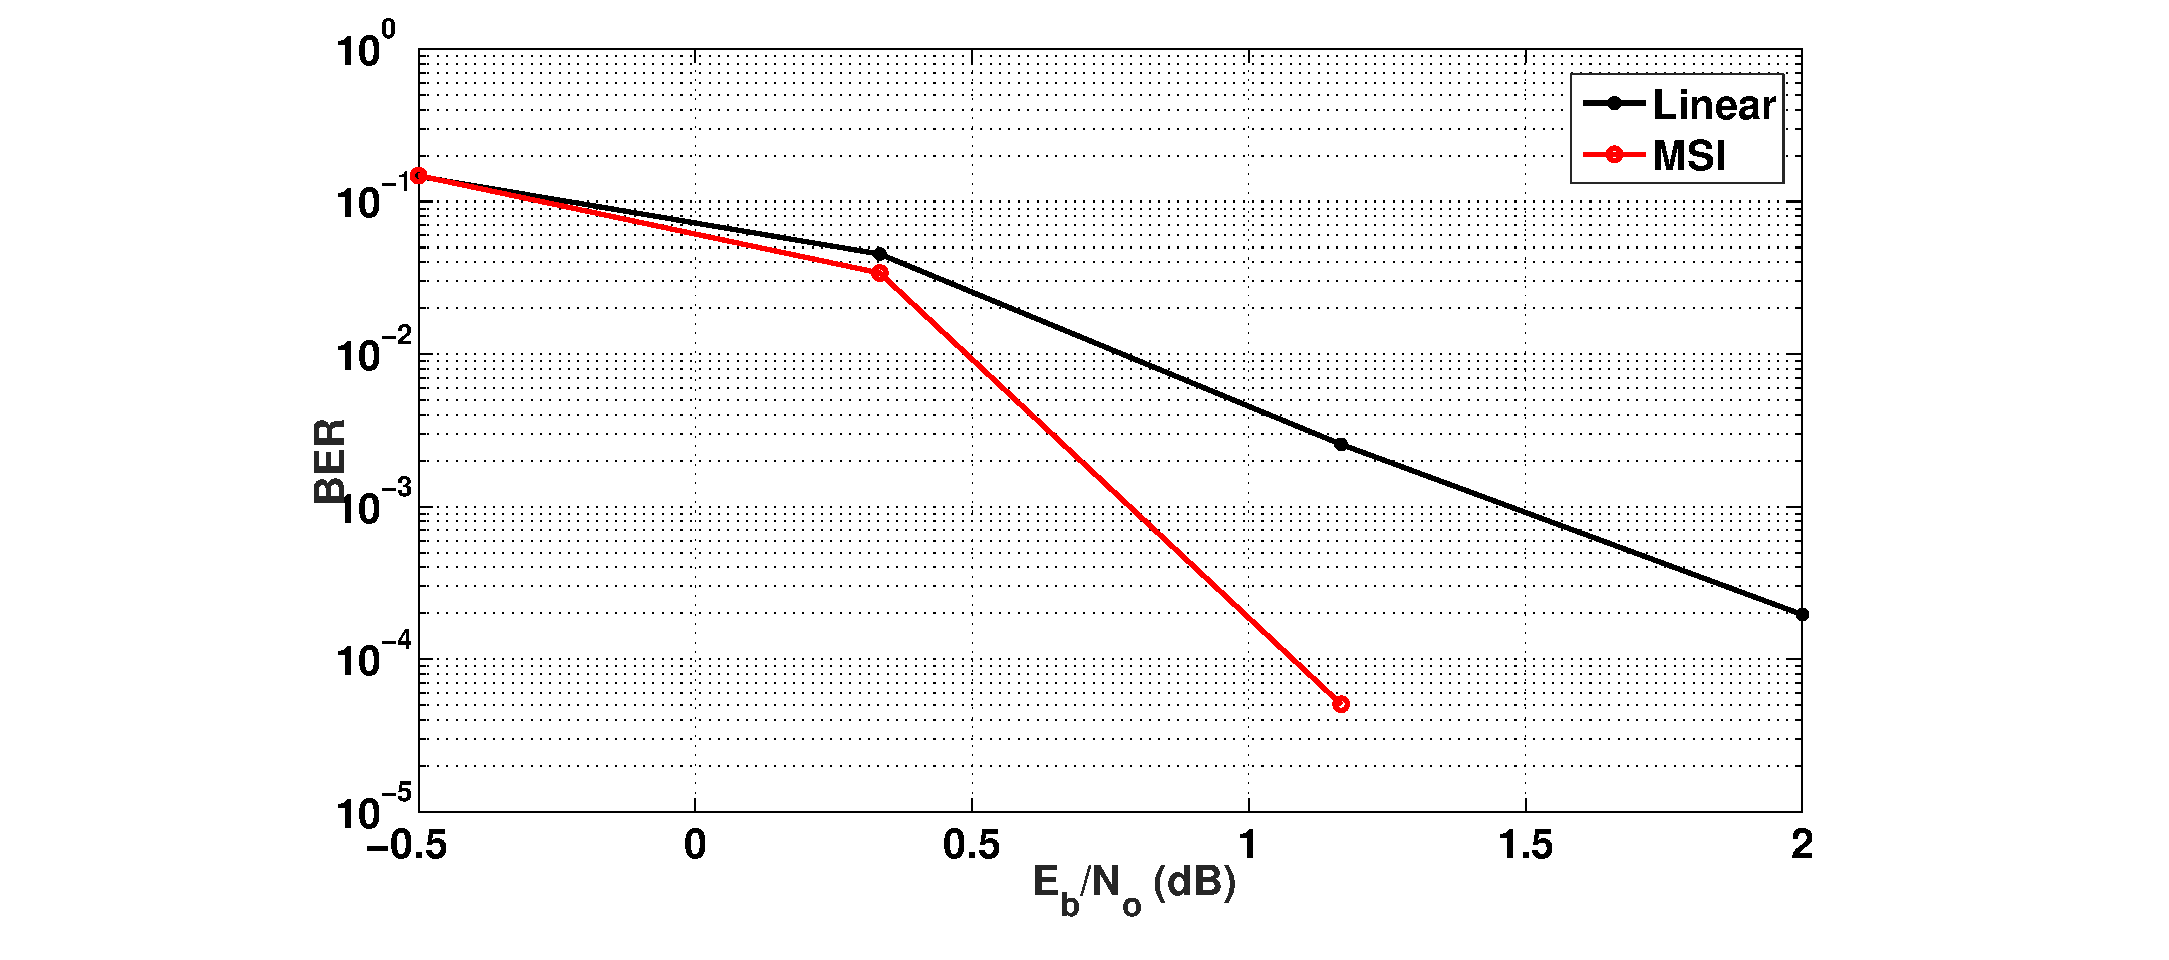
\includegraphics[width=8cm]{msi_linear_16384.eps}
\caption{$N=16384$, $D = d_0 =127$}
\label{y}
\end{figure}
\end{center}
\vspace{-8mm}
  The performance of the linear Interleaver as well as the multi-shift interleaver are compared via simulation. Interleaver length $N=1024$ and $N=16384$ are shown in figure \ref{x} and figure \ref{y} respectively. For medium and large frame sizes, the multi-shift interleaver outperforms the linear interleaver.
  \vspace{-4mm}
\section{Conclusion and Future Work}
In this research, the multi-shift interleaver was introduced. It outperforms the linear interleaver for both medium and long frame sizes. 

Future work include the comparison of the multi-shift interleaver to other interleavers and deriving theoretical BER upper bounds for the multishift interleaver.
\vspace{-4mm}
%%%%%%%%%%%%%%%%%%%%%%%%%%%%%%%%%%%%%%%%%%%%%%
\begin{thebibliography}{9}
\bibitem{ref2}Oscar Y. Takeshita, Member, IEEE, and Daniel J. Costello ,
''New Deterministic Interleaver Designs for Turbo Codes'',IEEE Trans. Inform. 
Theory, vol.  46,pp. 1988-2006,Nov. 2000.
\bibitem{ref5} Jing Sun, Oscar Y. Takeshita ''Interleavers for Turbo Codes Using 
Permutation Polynomials over Integer Rings'', IEEE Trans. Inform. Theory, vol. 51, 
pp. 101 - 119  Jan. 2005.
\end{thebibliography}



\end{document}
